\documentclass[letterpaper]{article}
\usepackage[margin=1in]{geometry}
\usepackage[utf8]{inputenc}
\usepackage{textcomp}
\usepackage{amssymb}
\usepackage{natbib}
\usepackage{graphicx}
\usepackage{gensymb}
\usepackage{amsthm, amsmath, mathtools}
\usepackage[dvipsnames]{xcolor}
\usepackage{enumerate}
\usepackage{mdframed}
\usepackage[most]{tcolorbox}
\usepackage{csquotes}
% https://tex.stackexchange.com/questions/13506/how-to-continue-the-framed-text-box-on-multiple-pages

\tcbuselibrary{theorems}

\newcommand{\R}{\mathbb{R}}
\newcommand{\Z}{\mathbb{Z}}
\newcommand{\N}{\mathbb{N}}
\newcommand{\Q}{\mathbb{Q}}
\newcommand{\C}{\mathbb{C}}
\newcommand{\code}[1]{\texttt{#1}}
\newcommand{\mdiamond}{$\diamondsuit$}
\newcommand{\PowerSet}{\mathcal{P}}
\newcommand{\Mod}[1]{\ (\mathrm{mod}\ #1)}
\DeclareMathOperator{\lcm}{lcm}

%\newtheorem*{theorem}{Theorem}
%\newtheorem*{definition}{Definition}
%\newtheorem*{corollary}{Corollary}
%\newtheorem*{lemma}{Lemma}
\newtheorem*{proposition}{Proposition}


\newtcbtheorem[number within=section]{theorem}{Theorem}
{colback=green!5,colframe=green!35!black,fonttitle=\bfseries}{th}

\newtcbtheorem[number within=section]{definition}{Definition}
{colback=blue!5,colframe=blue!35!black,fonttitle=\bfseries}{def}

\newtcbtheorem[number within=section]{corollary}{Corollary}
{colback=yellow!5,colframe=yellow!35!black,fonttitle=\bfseries}{cor}

\newtcbtheorem[number within=section]{lemma}{Lemma}
{colback=red!5,colframe=red!35!black,fonttitle=\bfseries}{lem}

\newtcbtheorem[number within=section]{example}{Example}
{colback=white!5,colframe=white!35!black,fonttitle=\bfseries}{def}

\newtcbtheorem[number within=section]{note}{Important Note}{
        enhanced,
        sharp corners,
        attach boxed title to top left={
            xshift=-1mm,
            yshift=-5mm,
            yshifttext=-1mm
        },
        top=1.5em,
        colback=white,
        colframe=black,
        fonttitle=\bfseries,
        boxed title style={
            sharp corners,
            size=small,
            colback=red!75!black,
            colframe=red!75!black,
        } 
    }{impnote}
\usepackage[utf8]{inputenc}
\usepackage[english]{babel}
\usepackage{fancyhdr}
\usepackage[hidelinks]{hyperref}

\pagestyle{fancy}
\fancyhf{}
\rhead{Math 170A}
\chead{Friday, February 03, 2023}
\lhead{Lecture 11}
\rfoot{\thepage}

\setlength{\parindent}{0pt}

\newcommand{\0}{\mathbf{0}}
\newcommand{\y}{\mathbf{y}}
\renewcommand{\b}{\mathbf{b}}
\newcommand{\x}{\mathbf{x}}
\newcommand{\e}{\mathbf{e}}
\newcommand{\rr}{\mathbf{r}}
\newcommand{\vv}{\mathbf{v}}
\renewcommand{\u}{\mathbf{u}}


\begin{document}

\section{Reduced QR (3.4)}
Let's begin with an example from a few sections ago. Suppose we have the following \textbf{full QR decomposition}
\begin{equation*}
    \begin{aligned}
        \underbrace{\begin{bmatrix}
            -1 & -1 & 1 \\ 
            1 & 3 & 3 \\ 
            -1 & -1 & 5 \\ 
            1 & 3 & 7
        \end{bmatrix}}_{A \in \R^{4 \times 4}} &= \begin{bmatrix}
            -\frac{1}{2} & \frac{1}{2} & -\frac{1}{2} & \frac{1}{2} \\ 
            \frac{1}{2} & \frac{1}{2} & -\frac{1}{2} & -\frac{1}{2} \\ 
            -\frac{1}{2} & \frac{1}{2} & \frac{1}{2} & -\frac{1}{2} \\ 
            \frac{1}{2} & \frac{1}{2} & \frac{1}{2} & \frac{1}{2}
        \end{bmatrix} \begin{bmatrix}
            2 & 4 & 2 \\ 
            0 & 2 & 8 \\ 
            0 & 0 & 4 \\ 
            0 & 0 & 0
        \end{bmatrix} \\ 
            &= \frac{1}{2} \underbrace{\begin{bmatrix}
                -1 & 1 & -1 & 1 \\ 
                1 & 1 & -1 & -1 \\ 
                -1 & 1 & 1 & -1 \\ 
                1 & 1 & 1 & 1
            \end{bmatrix}}_{Q \in \R^{4 \times 4}} \underbrace{\begin{bmatrix}
                2 & 4 & 2 \\ 
                0 & 2 & 8 \\ 
                0 & 0 & 4 \\ 
                0 & 0 & 0
            \end{bmatrix}}_{R \in \R^{4 \times 3}}.
    \end{aligned}
\end{equation*}
Here, $Q$ is orthogonal and $R$ is a tall matrix. Let's look at $R$. Notice how the last row of $R$ are just 0's. In particular, the last column of the matrix $Q$ and the last row of $R$ yields 0's everywhere; it's not helpful. So, what if we throw away the last row of $R$ and corresponding columns of $Q$? This brings us to the topic of \textbf{reduced QR}. In particular,
\[\underbrace{\begin{bmatrix}
    -1 & -1 & 1 \\ 
    1 & 3 & 3 \\ 
    -1 & -1 & 5 \\ 
    1 & 3 & 7
\end{bmatrix}}_{A \in \R^{4 \times 4}} = \frac{1}{2} \underbrace{\begin{bmatrix}
    -1 & 1 & -1 \\ 
    1 & 1 & -1 \\ 
    -1 & 1 & 1 \\ 
    1 & 1 & 1
\end{bmatrix}}_{\hat{Q} \in \R^{4 \times 3}} \underbrace{\begin{bmatrix}
    2 & 4 & 2 \\ 
    0 & 2 & 8 \\ 
    0 & 0 & 4
\end{bmatrix}}_{\hat{R} \in \R^{3 \times 3}}.\]
\textbf{Remark:} $\hat{Q}$ is not a square matrix anymore; it's a tall matrix. The concept of orthogonal matrices does not make sense here anymore. Instead, note that $\hat{Q}$ is an \textbf{isometry}; 
\[\underbrace{\hat{Q}^T}_{3 \times 4} \underbrace{\hat{Q}}_{4 \times 3} = \underbrace{I}_{3 \times 3}.\]
(Compare this to orthogonal, where we have $Q^T Q = QQ^T = I$.)

\begin{theorem}{Reduced QR}{}
    Suppose $A \in \R^{n \times m}$ such that $n \geq m$. Then, there exists a $\hat{Q} \in \R^{n \times m}$ isometry and $\hat{R} \in \R^{m \times m}$ upper-triangular such that \[A = \hat{Q}\hat{R}.\]
\end{theorem}
\textbf{Remark:} The reduced QR decomposition is unique if $\text{rank}(A) = m$ and we choose $r_{ii} > 0$ (entry on diagonal of $\hat{R}$). 


\subsection{Orthonormal Set}
Before we talk about how to obtain the reduced QR decomposition, we first introduce orthonormal sets. 
\begin{definition}{Orthonormal Set}{}
    We say that\footnote{Note that $q_i$ is a \emph{vector}.}
    \[\{q_1, q_2, \hdots, q_m\}\]
    is called \textbf{orthonormal} if $\cyclic{q_i, q_j} = 0$ whenever $i \neq j$ and $\cyclic{q_i, q_i} = 1$.
\end{definition}
\textbf{Remark:} If $Q$ is orthogonal (isometry), then the columns are orthonormal. For example, if the set $\{e_1, e_2\}$ is orthonormal, then this might visually look like 
\begin{center}
    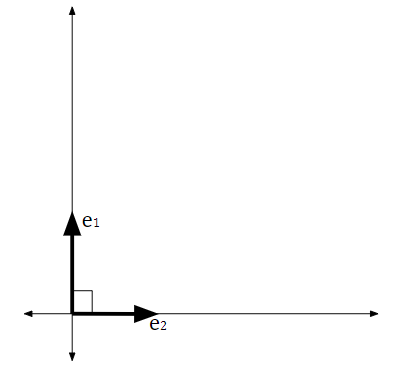
\includegraphics[scale=0.7]{../assets/orthonormal.png}
\end{center}

\subsection{Gram-Schmidt}
With the idea of orthonormal sets in mind, the idea is to use the \textbf{Gram-Schmidt} algorithm to make the columns of $A$ into an orthonormal set $\{q_1, q_2, \hdots, q_m\}$. This represents $\hat{Q}$. 

\bigskip 

Notationally, assuming $A$ has full rank (i.e., linearly independent), we can say that \[\{a_1, a_2, \hdots, a_m\}\] represents the columns of $A$. 


\subsubsection{Classical Algorithm}
Given $A$, we want to find $\hat{Q}$ and $\hat{R}$ such that $A = \hat{Q}\hat{R}$. As mentioned above, we can write $A$ as a set of linearly independent columns, 
\[\begin{bmatrix}
    a_1, a_2, \hdots, a_m
\end{bmatrix}.\]
We can also write $\hat{Q}$ in the same way:
\[\begin{bmatrix}
    q_1, q_2, \hdots, q_m
\end{bmatrix}.\]
We can write $\hat{R}$ like so: 
\[\begin{bmatrix}
    r_{11} & r_{12} & \hdots & r_{1m} \\ 
    0 & r_{22} & \hdots & r_{2m} \\ 
    \vdots & \vdots & \ddots & \vdots \\ 
    0 & 0 & \hdots & r_{mm}
\end{bmatrix}.\]
Combining this, we end up with 
\[\begin{bmatrix}
    a_1, a_2, \hdots, a_m
\end{bmatrix} = \begin{bmatrix}
    q_1, q_2, \hdots, q_m
\end{bmatrix} \begin{bmatrix}
    r_{11} & r_{12} & \hdots & r_{1m} \\ 
    0 & r_{22} & \hdots & r_{2m} \\ 
    \vdots & \vdots & \ddots & \vdots \\ 
    0 & 0 & \hdots & r_{mm}
\end{bmatrix}.\]
Then, we note that 
\[a_1 = q_1 r_{11} \implies q_1 = \frac{a_1}{r_{11}} \implies r_{11} = ||a_1||_2.\]
\[a_2 = q_1 r_{12} + q_2 r_{22}.\]
\[a_3 = q_1 r_{13} + q_2 r_{23} + q_3 r_{33}.\]
Eventually, we'll end up with 
\[a_m = q_1 r_{1m} + q_2 r_{2m} + \hdots + q_m r_{mm}.\]
So, this is the basic idea: processing each column one at a time. Writing this out as steps, we have: 
\begin{enumerate}
    \item $r_{11} = ||a_1||_2$, $q_1 = \frac{a_1}{r_{11}} = \frac{a_1}{||a_1||_2}$. It follows that \[||q_1||_2 = 1.\]
    \item $a_2 = r_{12}q_1 + r_{22}q_2$. Then, we can multiply $q_1$ on both sides: 
    \begin{equation*}
        \begin{aligned}
            \cyclic{a_2, q_1} &= \cyclic{r_{12}q_1 + r_{22}q_2, q_1} \\ 
                &= r_{12}\underbrace{\cyclic{q_1, q_1}}_{1} + r_{22} \underbrace{\cyclic{q_2, q_1}}_{0} \\ 
                &= r_{12}.
        \end{aligned}
    \end{equation*}
    Note that we got the 0 and 1 from the properties of orthonormal sets. In any case, it follows that \[q_2 = \frac{a_2 - r_{12}q_1}{r_{22}}.\]
    Setting $r_{22} = ||a_2 - r_{12}q_1||_2$, it follows that $||q_2||_2 = 1$. 

    \item We start from $a_3$ and determine $q_3$ and $r_{13}$, $r_{23}$, and $r_{33}$. 
\end{enumerate}
Notice that we essentially keep going like this. Let's try to generalize this. The formula for $\hat{R}$ is given by 
\[\hat{R} = (r_{ji})\]
for $j < i$. Then, \[\hat{Q} = \begin{bmatrix}
    q_1 & q_2 & \hdots & q_m
\end{bmatrix}\] and we can get $A = \hat{Q} \hat{R}$. Remember that 
\[r_{12} = \cyclic{a_2, q_1}.\] Note that the 1 in $r$ index corresponds to the 1 in $q_1$ and the 2 in the $r$ index corresponds to the 2 in $a_2$. We also know that 
\[r_{22} = ||a_2 - r_{12}q_1||_2\] and 
\[q_2 = \frac{a_2 - r_{12}q_1}{r_{22}}.\]
Analogously, notice that 
\[r_{13} = \cyclic{a_3, q_1}\] and \[r_{23} = \cyclic{a_3, q_2}.\] We also know that \[a_{33} = ||a_3 - r_{13}q_1 - r_{23}q_2||_2\] and \[q_3 = \frac{a_3 - \sum_{j = 1}^{2} r_{j3} q_j}{r_{33}}.\] 
\underline{So, to conclude, we can generalize the formula:}
\[r_{ii} = \left|\left| a_{i} - \sum_{j = 1}^{i - 1} r_{ji} q_j \right|\right|_2.\]
\[r_{ji} = \cyclic{a_i, q_j} \qquad j < i.\]
\[q_i = \frac{a_i - \sum_{j = 1}^{i - 1} r_{ji} q_j}{r_{ii}}.\]

\end{document}